\documentclass[12pt]{article}
\usepackage{ctex}
\usepackage{amssymb}
\usepackage{mathrsfs}
\addtolength{\topmargin}{-.5in} \addtolength{\textheight}{1in}
\addtolength{\oddsidemargin}{-.6in}
\addtolength{\evensidemargin}{-.6in} \addtolength{\textwidth}{1.2in}
\usepackage{latexsym,amsmath,amssymb,amsfonts,epsfig,graphicx,cite,psfrag}
\usepackage{eepic,color,colordvi,amscd}
\usepackage{latexsym,amssymb,amsfonts,epsfig,graphicx,cite,psfrag}
\usepackage{eepic,color,colordvi,amscd}
\usepackage{siunitx,booktabs,cancel,caption,cleveref,colortbl,csquotes,multirow,listings,xcolor}
\usepackage{float}
\usepackage{subfig}
\usepackage{amsmath}
\usepackage{nth}
\usepackage[justification=centering]{caption}
\usepackage[final]{hyperref}
\def\qed{\hfill \rule{4pt}{7pt}}

\pagestyle{plain}

\begin{document}

\title{\textbf{第八次实验报告:贪心算法}}
\author{\textbf{陈潇涵}\space \textbf{PB13000689}}
\date{\textbf{2016\space 年\space 5\space 月 \space 5\space 日}}
\maketitle

\section*{实验内容}
本次实验通过实现最短路径的Dijkstra算法和最小生成树的Prim算法和Kruskal算法,来
加深对贪心算法的理解。

\section*{实验原理}
\subsection*{单源最短路径的Dijkstra算法}
单源最短路径的Dijkstra算法中有两个集合,一个是已经求得最短路径的顶点集合S,另一
个是还需求解最短路径的顶点集合Q。在每一步选择,都是在第二个集合中选择路径最短的
一个,加到集合S中,并从集合Q中去掉。然后在以这一个点为依据更新第二个集合中的所
有点的最短距离。直到第二个集合为空。

\medskip

\textbf{正确性}:可以用反证法证明对从起点s到终点t的最短路径上的每个顶点v,该路
径都是从s到v的最短路径。否则,我们可以找到更短的一条从s到v的路径,再加上从v到t
的路径,就得到了从s、到t的一条更短路径。

\medskip

\textbf{贪心法则的正确性}:假设集合Q中的距离最短的点为u,最短距离为d,即,从源
点s出发经过集合S到顶点u的最短距离为d。而从源点s到Q中其它点v的距离都大于d,因此
每一条经过v再到达u的路径长度都大于d。因此d一定是从s到达u的最短距离,此时选择u加
入集合S一定是安全的。

\subsection*{MST的Kruskal算法}
Kruskal算法我觉得还是很好理解的:我们将所有顶点初始化为一个只包含自己的集合,再
将所有边按照权重由低到高的顺序进行排序。从排好序的边中我们一条条取出来,如果这条
边连接的两个顶点所在的集合相同,即表示这两个顶点已经是连通的了,那么我们不做任何
操作;如果这条边的两个端点所在的集合不同,则说明这两个顶点不连通,于是我们将这条
边加入到最小生成树的边集合中。重复以上过程知道边集合的大小等于顶点集大小减一。

\medskip

\textbf{正确性}:然而严格的正确性听韩路新说要用拟阵什么的去证明,于是我一脸懵逼。
因为在我看来这个方法的正确性是不言自明的……

\medskip

\textbf{时间复杂度}:Kruskal算法的时间复杂度取决于连通子集的数据结构。如果用书
上21章第3节的高级方法,|V|个顶点的Make-Set方法和|E|次循环中的Find-Set和Union方
法,根据21.3中的结论可以得到总的时间复杂度为$ O((E+V)\alpha(V)) $,其中
$ \alpha(V) $是一个随V增长非常缓慢的函数。再考虑一下图的连通性,有$ E\geq V-1 $
以及$ E \leq V^2 $,我们有总的时间复杂度为 $ O(E\log{V}) $。但是我用python写的
时候用了一些python的特性,同样能达到上述复杂度,我会在后面实验内容中再详细说明。

\subsection*{MST的Prim算法}
Prim算法也很好理解。Prim算法中维持两个集合和一些信息:第一个集合S是已经确定加入
最小生成树的顶点集合,第二个集合Q是还需确认的顶点集合,算法执行过程中我们还需要
维护Q集合中的顶点u的信息——u到集合S的距离。

\medskip

\textbf{贪心法则}:每一次我们都选择到集合S距离最短的点u加入集合S,再从集合Q中
删除。之后我们再更新Q中顶点到集合S的距离。重复上述步骤直到集合Q为空。

\medskip

\textbf{正确性}:假设某一步贪心选择中选取的边不是任何一棵最小生成树的边。假设
最终生成的最小生成树中集合S通过路径 $S-u_1-u_2-\ldots -u_m-u$使得集合S与顶点u
连通,且$u_1,u_2,\ldots,u_t$都是集合Q中的点,由于u是距离集合S最近的点,我们将
边$S-u_1$替换为边$S-u$,这样我们得到的仍然是一棵生成树,且这棵生成树的代价比原
来的生成树小,这与原来的生成树是最小生成树的假设想矛盾。Prim算法的正确性由此得
证。

\medskip

\textbf{时间复杂度}:Prim算法的时间复杂度决定于集合Q中最小距离顶点选取的实现方
式。如果我们用堆排序中的方法将集合Q维持成最小堆的形态,然后在每一次选取u的时候
选取根即可,从u中删除点时只需要将根与对中最后一个元素互换,然后维持一下堆的性质
,这个操作的时间复杂度是$ \log{V} $。在初始化步骤我们需要建立最小堆,这里的时
间复杂度是$ O(V) $。Prim算法中的循环部分需要执行V次,因此提取最小元素部分的操
作的时间复杂度共需要$ O(V\log{V}) $。Prim算法中,更新距离的操作的执行次数之多
不超过$ 2E $次,每一次更新操作中,判断点在Q中可以在常数时间内完成,如果我们开
辟一个数组来额外记录每个顶点是否在Q中即可;修改距离后,我们还需要维持最小堆性质
,时间复杂度为$ \log{V} $。因此更新距离的总时间复杂度为$ O(E\log{V}) $。因此,
Prim算法的总时间复杂度为

$$ O(V\log{V})+O(E\log{V}) = O(E\log{V})) .$$

\section*{实验中出现的问题}
实验中没有出现什么问题。

\section*{实验内容}

\begin{figure}[H]
    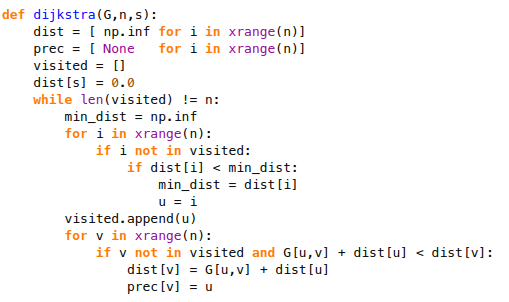
\includegraphics[width=0.60\textwidth]{dijkstra_code.png}
    \caption{Dijkstra 算法代码截图}
\end{figure}

\begin{figure}[H]
    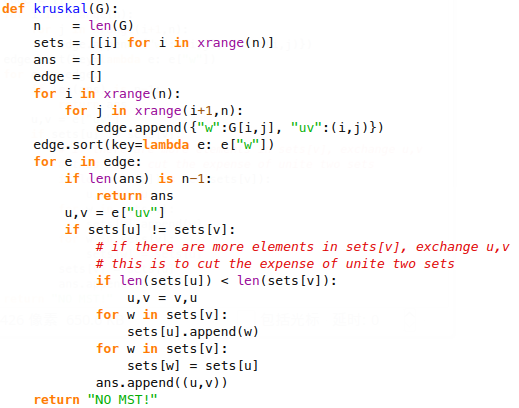
\includegraphics[width=0.65\textwidth]{kruskal_code.png}
    \caption{Kruskal 算法代码截图}
\end{figure}

\begin{figure}[H]
    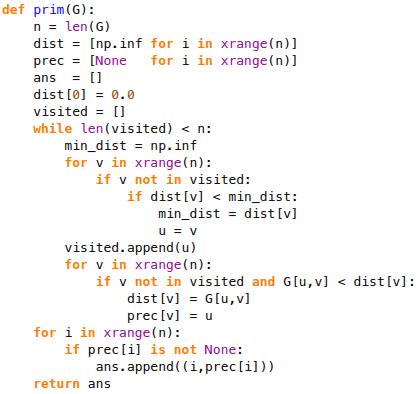
\includegraphics[width=0.60\textwidth]{prim_code.png}
    \caption{Prim 算法代码截图}
\end{figure}

说明,这里我的Prim算法并没有用最小堆来做(懒得做了……)。

\medskip

来我们来看一下我写的Kruskal算法的部分。初始化时我用python中的list对象来表示连通
的子集,于是每一个顶点v,对应的初始集合是$[v]$。edge是边集,我用python内置的sort
方法对edge按权重进行由低到高的排序。对于排序好的edge中的每一条边e,我先得到了e的
两个端点u,v。我们先判断是否有$sets[u] = sets[v]$(这里的正确性我们等会再说)
。如果相等,表示u和v已经是连通的了,这条边不需要再加进来。如果不相等,那么我们把
这条边加到最小生成树的边集中去(即ans集合)。然后进行对u和v所在的集合进行合并。
合并分为四步。第一步,判断$sets[u],sets[v]$的长度,如果后者大,交换u,v。这一步
的目的在于保证我们每一步都是较短集合加入较长集合。第二步,讲$sets[v]$中的每一个
元素w都加入到$sets[u]$中,表示实际的集合合并过程。第三步,将$sets[u]$的值赋给
$sets[v]$中的每一个元素w,$sets[w]=sets[u]$。注意,这里是重点。我们不需要对
$sets[u]$中的所有其它元素对应的连通子集进行改变,原因是,python中的有一个特性
,它里面的任何变量都是一个引用。我们在进行对$sets[u]$进行append操作时,已经对
和u连通的顶点对应的sets进行了改变,通过这一点点特性,我们可以讲这部分的总时间复杂
度变为$V\log{V}=E\log{V}$。

\section*{实验分析}

\begin{figure}[H]
    \centering
    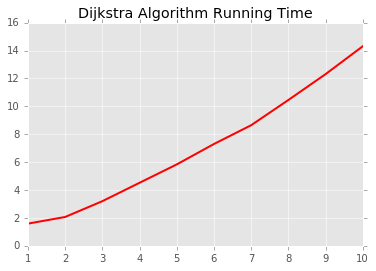
\includegraphics[width=0.70\textwidth]{dijkstra.png}
    \caption{Dijkstra算法运行时间图:$ \log{T}-\log{n} $}
\end{figure}

\begin{figure}[H]
    \centering
    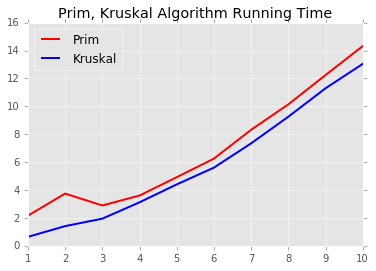
\includegraphics[width=0.70\textwidth]{mst.png}
    \caption{Prim,Kruskal算法运行时间图}
\end{figure}

从实验结果可以看到,这几个算法的运行时间的对数和顶点数的对数基本上成线性关系,
斜率差不多为1.3左右,这和理论上的时间复杂度还是比较契合的。

\medskip

Kruskal算法始终要比Prim算法要快一些,我猜测原因是我的prim算法没有用到堆来进行
贪心选择,导致时间复杂度比Kruskal要高。

\section*{实验总结}

这次实验做的还是蛮愉快的,对这几个经典算法有了更深得了解,对python的一些特性也
多了一些了解。

\end{document}